Our main research question is defined in the following way:

\begin{quote}
How do organizations perform information security incident management in practice?
\end{quote}

This is a so-called "how" question. Figure \ref{fig:methods} shows an overview of various research methods and three criteria that can be used to determine which method to choose. Based on the type of research question this study has, several of this methods could have been chosen. However, our study focuses on contemporary events, as we wish to examine incident handling in practice in the present time, and not from a historical point of view. Additionally the goal is to examine practices in organizations and we do not require control of behavioural events. Based on figure \ref{fig:methods}, case study emerged as the most suitable method for this study.

\begin{figure}[H]
%\hspace*{-0.4cm}
\begin{center}
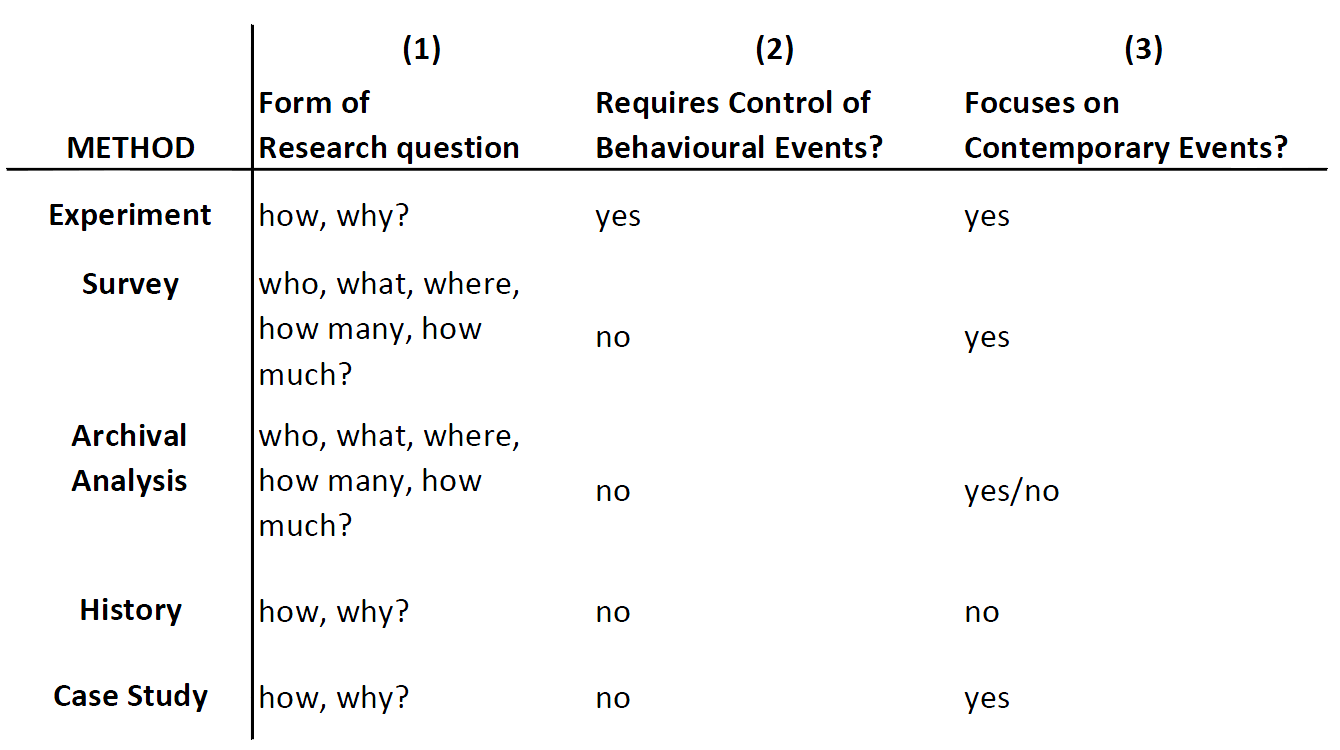
\includegraphics[scale=0.35]{methods.png}
\caption[Situations for different research methods]{Situations for different research methods, derived from \cite{CaseStudyResearch}}
\label{fig:methods}
\end{center}
\end{figure}